\documentclass[tikz,border=3.14mm]{standalone}
\usetikzlibrary{matrix,fit,positioning,snakes}
\tikzset{
mymat/.style={
    matrix of math nodes,
    left delimiter=|, right delimiter=|,
    align=center,
    toprule,
    column sep=-\pgflinewidth
},
mymats/.style={
    mymat,
    nodes={draw,fill=#1}
}  ,
toprule/.style={%
        execute at end cell={%
            \draw [line cap=rect,#1, dashed] (\tikzmatrixname-\the\pgfmatrixcurrentrow-\the\pgfmatrixcurrentcolumn.north west) -- (\tikzmatrixname-\the\pgfmatrixcurrentrow-\the\pgfmatrixcurrentcolumn.north east);%
        }
    },
} 

\begin{document}
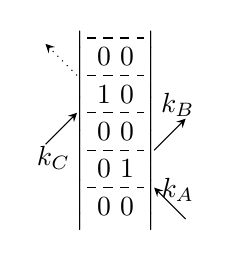
\begin{tikzpicture}[%font=\sffamily,
    every left delimiter/.style={xshift=.4em},
    every right delimiter/.style={xshift=-.4em}]
% first diagram
\matrix[mymat] at (0,0) (mat1)
{   0  0\\
    1  0\\
    0  0\\
    0  1\\
    0  0\\
};
\draw[stealth-] (mat1-4-1.south -| mat1.east) -- ++(4mm,-4mm) node[pos=0.75,above]{$k_A$};
\draw[-stealth] (mat1-3-1.south -| mat1.east) -- ++(4mm,4mm) node[pos=0.75,above]{$k_B$};
\draw[stealth-] (mat1-2-1.south -| mat1.west) -- ++(-4mm,-4mm) node[pos=0.75,below]{$k_C$};
\draw[-stealth, dotted] (mat1-1-1.south -| mat1.west) -- ++(-4mm,4mm) ; %node[pos=0.75,below]{$k_S$};

\end{tikzpicture}
\end{document}